\chapter{Architecture}
\label{chap-dev}
\label{chap-description-src}

\renewcommand{\headrulewidth}{0.3pt}
\fancyhead[LE]{\thepage} \fancyhead[RE]{\nouppercase{\textbf{\leftmark}}}
\fancyhead[RO]{\thepage} \fancyhead[LO]{\nouppercase{\textbf{\rightmark}}}
\fancyfoot[L,C,R]{}

\setlength{\parindent}{0.35cm}

\minitoc
\newpage
% ================================================================

Ce chapitre décrit l'architecture conceptuelle --- la séparation HTAS/CWV et les trois couches du backend --- ainsi que les \textbf{règles} qu'un développeur doit suivre en travaillant au sein de cette structure, et les deux portes d'entrée par lesquelles doivent passer tous les appels frontend~$\rightarrow$~backend. Les recettes concrètes d'extension de l'application et l'outillage associé suivent dans les chapitres suivants.

\section{Architecture séparée : HTAS et CWV}
\label{sec-split}

\cwv~est construit au-dessus d'un backend scientifique autonome qu'il consomme au travers d'une interface publique bien définie. Comprendre le code revient donc à comprendre deux choses : comment l'application QGIS et le backend sont maintenus \emph{séparés}, et comment le backend est organisé en interne en \emph{trois couches}. Cette section décrit les deux, et énonce les règles strictes qu'un développeur doit suivre en travaillant au sein de cette structure.

\cwv~est maintenu sous forme de deux paquets gardés \textbf{strictement indépendants} :

\begin{itemize}
    \item \textbf{\script{HydrologicalTwinAlphaSeries} (HTAS)} --- le backend scientifique autonome : traitement des simulations, structures du domaine (compartiments, maillages, observations), modèles de configuration, et la façade \script{HydrologicalTwin}. Il réside sous \script{external/HydrologicalTwinAlphaSeries} ; dans la configuration publiée, ce chemin est un sous-module \gitlab~pointant vers le dépôt du backend autonome.
    \item \textbf{\script{cawaqsviz} (CWV)} --- l'application QGIS autonome : boîtes de dialogue, flux de visualisation, intégration SIG, et adaptateurs côté application.
\end{itemize}

L'indépendance est un \textbf{invariant} architectural strict, et non une préférence de style :

\begin{itemize}
    \item HTAS ne doit \textbf{jamais} importer \script{qgis.*}, \script{PyQt5}, \script{processing}, ni quoi que ce soit depuis \script{cawaqsviz/}. Si vous vous apprêtez à ajouter un tel import à l'intérieur de \script{external/HydrologicalTwinAlphaSeries/}, arrêtez --- le travail relève du côté CWV ;
    \item \cwv~ne doit consommer HTAS qu'à travers son API publique --- les deux portes d'entrée (\cref{sec-dev-gates}) --- et garder le code d'adaptation propre à QGIS côté application. Les imports HTAS à l'exécution relèvent de \script{interface/} ; les modules \script{frontend/} n'accèdent au comportement du backend qu'à travers la passerelle de l'application ;
    \item le backend est conçu pour être \textbf{utilisable depuis un notebook aujourd'hui et un serveur demain} (\cref{sec-notebook-usage}). Tout ce qui casse l'usage depuis un notebook en Python pur casse aussi le futur serveur ;
    \item la synchronisation entre les deux dépôts se fait par le contrôle de version et l'épinglage des dépendances, non par duplication de code.
\end{itemize}

\begin{figure}[htbp]
    \centering
    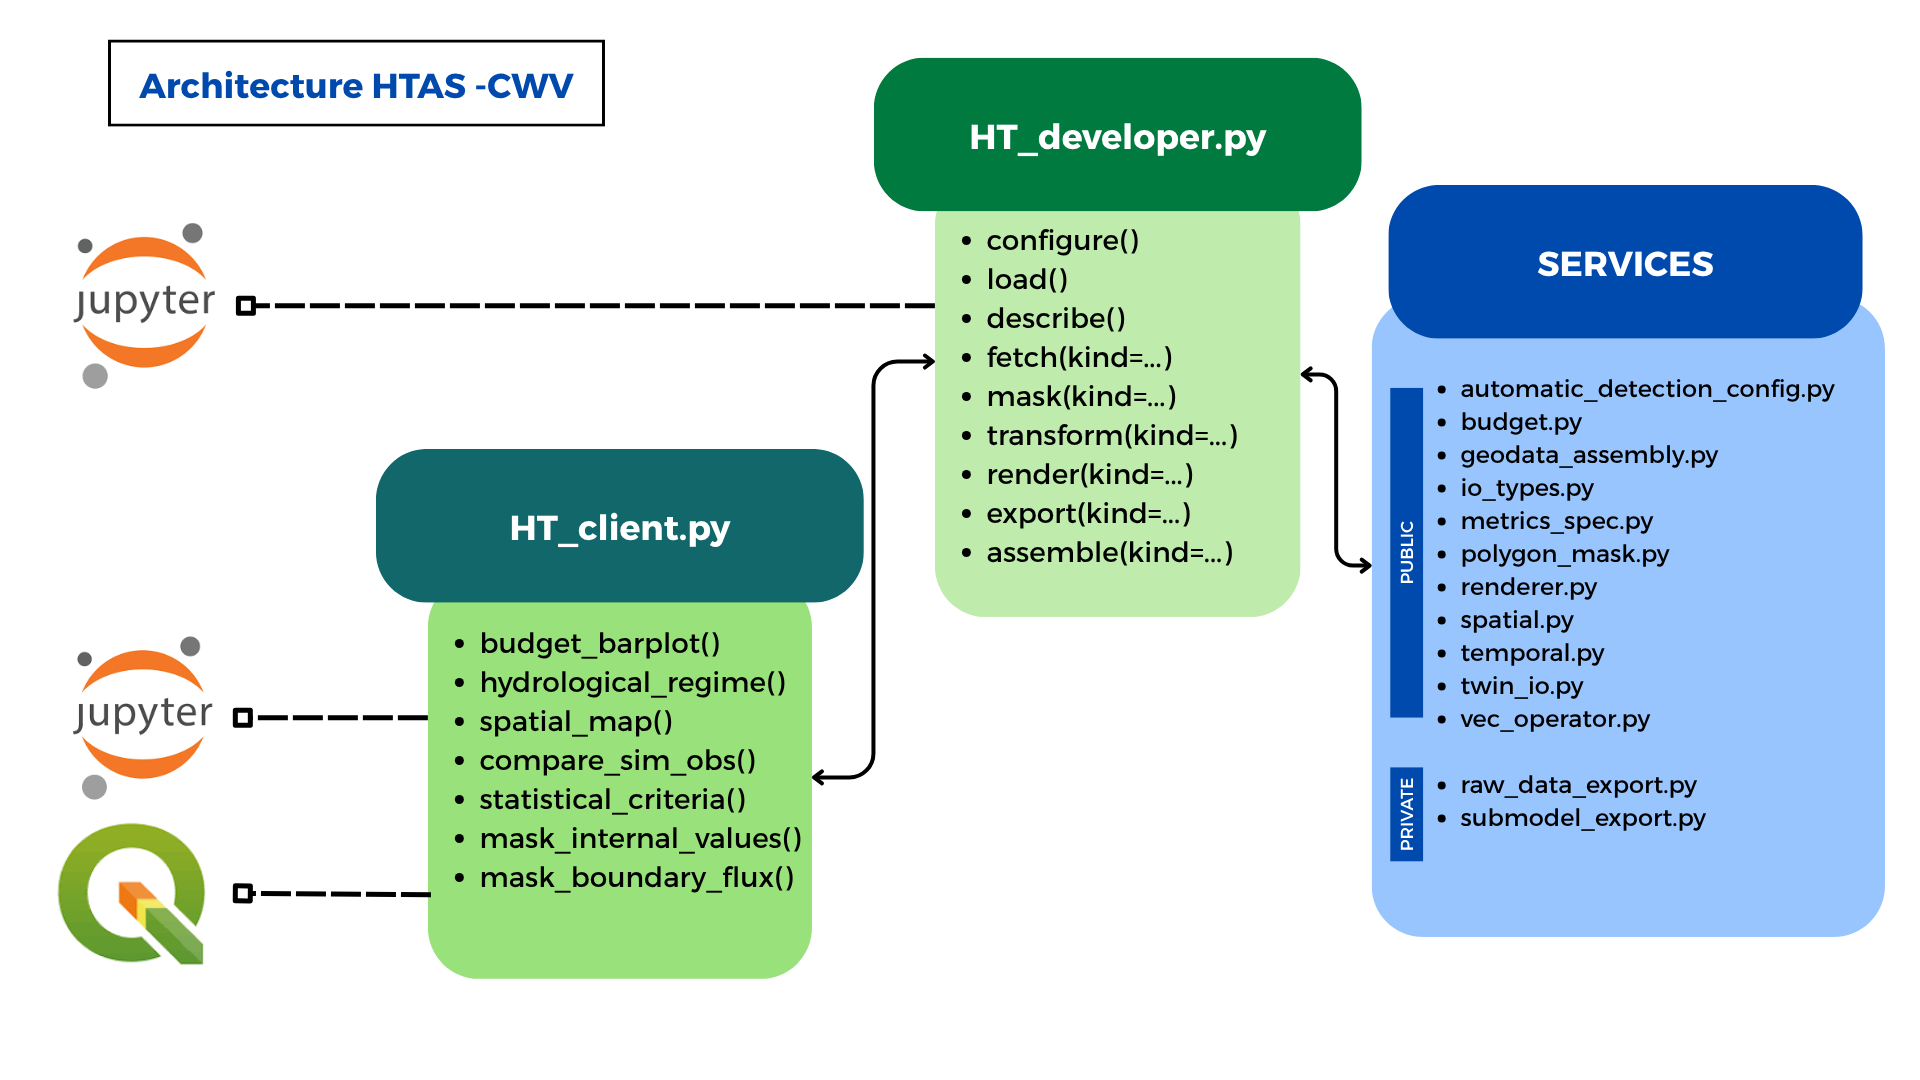
\includegraphics[width=\linewidth,height=0.85\textheight,keepaspectratio]{7_architecture/fig/architecture_developer_overview.png}
    \caption{Architecture \cwv~+~HTAS. Les trois couches du backend sont L1 (\script{HT\_Client}), L2 (\script{HT\_developer}), et L3 (\script{Services}).}
    \label{fig-architecture-overview}
\end{figure}

\section{Les trois couches du backend}
\label{sec-layers}

HTAS est organisé selon une \textbf{architecture à trois niveaux} dans laquelle chaque niveau peut appeler le niveau inférieur, jamais le niveau supérieur. Chaque niveau possède un module d'entrée canonique, et les imports pointent \textbf{strictement vers le bas} (L1~$\rightarrow$~L2~$\rightarrow$~L3) : jamais vers le haut, jamais latéralement au sein d'un niveau. Comme chaque dépendance pointe vers le bas, les couches ne peuvent jamais former une boucle d'import --- le graphe de dépendances est acyclique.

\begin{lstlisting}[language=bash, caption={Les trois couches du backend et leurs modules d'entrée canoniques.}, label={code-layers}]
L1 - HT CLIENT - MACRO        ht/client/hydrological_twin_client.py       (peut importer L2, L3)
L2 - HT DEVELOPER - MICRO     ht/developer/hydrological_twin_developer.py (peut importer L3)
L3 - SERVICES - ELEMENTARIES  services/                                   (n'importe rien dans ht/)
\end{lstlisting}

Avec les couches côté QGIS (frontend et interface), les rôles sont résumés dans le \cref{tab-layers}.

\renewcommand{\arraystretch}{1.3}
\begin{table}[H]
    \centering
    \begin{tabularx}{\linewidth}{>{\raggedright\arraybackslash}m{3.6cm}|X}
        \hline
        \textbf{Couche} & \textbf{Rôle} \\
        \hline
        \textbf{Frontend} \newline \script{frontend/} & Boîtes de dialogue QGIS. Elles gèrent l'interaction utilisateur et acheminent un unique appel grossier par flux vers l'interface. \script{Qt}/\script{PyQt5} vit ici et seulement ici. \\
        \hline
        \textbf{Interface} \newline \script{interface/} & \script{ExploreData} est la \textbf{seule} passerelle vers le backend ; \script{GeoDataProvider} transforme les couches vectorielles QGIS en \script{GeoDataFrame} pour que le backend reste agnostique de QGIS. \\
        \hline
        \textbf{L1 - HT CLIENT - MACRO} \newline \script{ht/client/} & \script{HydrologicalTwinClient} expose une méthode par opération de dialogue orientée utilisateur. Chacune délègue à un \script{operations\_client.run\_*} correspondant qui possède toute la chaîne \script{fetch}~$\rightarrow$~\script{transform}~$\rightarrow$~\script{render} et renvoie une dataclass typée \script{*Result}. Zéro import \script{qgis}/\script{PyQt5} --- utilisable depuis un notebook aujourd'hui, depuis un serveur HTTP demain. \\
        \hline
        \textbf{L2 - HT DEVELOPER - MICRO} \newline \script{ht/developer/} & \script{HydrologicalTwin} est la façade micro-verbes exposant 8 verbes canoniques avec une machine à états explicite \script{EMPTY}~$\rightarrow$~\script{CONFIGURED}~$\rightarrow$~\script{LOADED}~$\rightarrow$~\script{READY}. Utile pour l'exploration en notebook et pour les opérations pas encore promues au client. \\
        \hline
        \textbf{L3 - SERVICES - ELEMENTARIES} \newline \script{services/} & Calculs et E/S les plus fins : opérateurs, moteur de rendu, lectures d'état du jumeau et provisionnement du cache disque (\script{twin\_io.py}), et DTO de données feuilles (\script{io\_types.py}). Aucun module sous \script{services/} n'importe depuis \script{ht/} --- le graphe d'import est un DAG strictement descendant et acyclique. \\
        \hline
    \end{tabularx}
    \caption{Rôles du frontend, de l'interface et des trois couches du backend.}
    \label{tab-layers}
\end{table}

\script{ExploreData} appelle \textbf{le client} pour les opérations grossières (la voie normale) et peut encore atteindre le jumeau développeur \textit{via} \script{client.\_twin} pour des appels micro-verbes de bas niveau. Une vue plus annotée du flux de données est donnée dans le \cref{fig-architecture-overview}.

\textbf{Règle d'or --- les imports pointent uniquement vers le bas.} Jamais vers le haut, jamais latéralement au sein d'un niveau. Aucun module sous \script{services/} ne peut importer depuis \script{ht/client/} ou \script{ht/developer/}. Les DTO de données partagés vivent à la feuille L3 (\script{services/public/io\_types.py}) et sont ré-exportés par le \script{api\_types.py} de L2, de sorte que l'arête reste descendante. Comme chaque dépendance pointe vers le bas, le graphe ne peut jamais former de boucle d'import --- c'est un DAG strictement descendant et acyclique.

\textbf{Règle d'or (corollaire) --- L1 ne fait qu'orchestrer, il ne manipule pas les données.} L1 (\script{hydrological\_twin\_client.py} et, derrière lui, \script{operations\_client.py}) est de l'\emph{orchestration pure} : il ne peut qu'\emph{appeler} des micro-verbes L2 et \emph{regrouper} leurs résultats typés dans une dataclass \script{*Result}. Il ne doit contenir \textbf{aucune manipulation de données propre} --- pas de construction de \script{DataFrame}, pas de remise en forme ou d'agrégation de tableaux, pas de mise en forme d'unités/chemins/provenance, pas d'E/S disque, pas de calcul du domaine. Toute logique de ce type relève d'un cran plus \emph{bas}, dans un micro-verbe L2 (\script{fetch}/\script{transform}/\script{render}/\script{export}, ou un nouveau \script{kind=}) ou dans L3 \script{services/}. Le test : si une ligne dans \script{ht/client/} fait autre chose qu'appeler une couche inférieure ou empaqueter/désempaqueter un résultat typé, elle est dans la mauvaise couche.

\alertwarning{Le code assume d'être en transition : la flèche propre L2~$\rightarrow$~L3 unique décrite ici est la \emph{cible}, pas encore le code littéral. Deux réserves sur l'état actuel qu'un développeur doit garder à l'esprit : (i)~au sein de L2, \script{ht/developer/dispatch.py} et \script{ht/developer/handlers.py} sont des modules \textbf{transitoires} internes à L2 --- aujourd'hui les micro-verbes routent \script{hydrological\_twin\_developer.py}~$\rightarrow$~\script{dispatch.py}~$\rightarrow$~\script{handlers.py} avant d'atteindre L3, et ces deux modules sont destinés à être fondus dans les corps des micro-verbes L2 (voir \script{external/HydrologicalTwinAlphaSeries/docs/TODO.md}) ; (ii)~quelques imports descendants entre couches (par ex.\ la réutilisation de la fonction de récupération de la matrice de simulation à l'intérieur de plusieurs méthodes L2) sont tolérés pour l'instant et seront resserrés plus tard --- ils ne posent actuellement pas de problème pour l'usage en notebook.}

\section{Exemple de flux de travail : le Budget Bar Plot}
\label{sec-example-workflow}

Le déroulé suivant montre ce qui se passe, pas à pas, lorsqu'un utilisateur crée un histogramme de bilan hydrique. C'est l'un des flux les plus complets, enchaînant \script{fetch}~$\rightarrow$~\script{transform}~$\rightarrow$~\script{render}, et il est utile pour comprendre le nombre d'allers-retours entre couches --- en particulier lors de la conception de la future API serveur.

\begin{enumerate}
    \item Dans la boîte de dialogue \script{DialogBudgetbarplot}, l'utilisateur sélectionne des variables, une période, une fréquence et une agrégation.
    \item La boîte de dialogue émet un \emph{unique} appel grossier vers \script{ExploreData}, qui le transmet à \script{HydrologicalTwinClient.budget\_barplot(**kwargs)}, lequel appelle à son tour \script{operations\_client.run\_budget\_barplot}.
    \item Pour chaque variable (pluie, ETR, infiltration, ruissellement), l'orchestration appelle \script{twin.fetch} (lit la matrice de simulation depuis le disque à travers la couche services) puis \script{twin.transform} (moyenne spatiale + agrégation temporelle).
    \item Un dernier appel \script{twin.render} produit le tracé ; le moteur de rendu écrit un PNG et un CSV sur le disque et renvoie leurs chemins.
    \item Les chemins sont regroupés dans une dataclass \script{BudgetBarplotResult} et remontés le long de la chaîne jusqu'à la boîte de dialogue, qui ouvre le fichier du tracé.
\end{enumerate}

Ce que cela révèle pour la conception de l'API :

\begin{itemize}
    \item aujourd'hui, tout ce qui se trouve entre \script{ExploreData} et le jumeau développeur est \textbf{en processus}. La couture réseau naturelle est la frontière \script{ExploreData}~$\rightarrow$~\script{Client}, pas \script{ExploreData}~$\rightarrow$~\script{HydrologicalTwin} ;
    \item \textbf{une opération grossière = un aller-retour serveur}. La boîte de dialogue appelle \script{client.budget\_barplot(...)} une fois ; la boucle interne de 4 fetches + 4 transforms + 1 render reste côté serveur à l'intérieur de \script{run\_budget\_barplot}. L'ancien coût de « 9 appels par tracé » s'effondre en un seul appel à la frontière réseau ;
    \item \textbf{le client \emph{est} la future surface HTTP.} Chaque méthode de \script{HydrologicalTwinClient} correspond proprement à un point de terminaison, avec une dataclass typée \script{*Result} comme schéma de réponse. L'API micro-verbes développeur reste disponible pour l'exploration façon notebook ;
    \item \textbf{le rendu écrit encore sur le disque.} Lorsque le client passera côté serveur, les sorties de rendu devront renvoyer des données (ou des URL signées) plutôt que des chemins de fichiers locaux --- les dataclass \script{*Result} sont le bon endroit pour faire évoluer ce contrat.
\end{itemize}

\section{Portes d'entrée}
\label{sec-dev-gates}

Tous les appels frontend~$\rightarrow$~backend passent par l'une de deux surfaces. Ne les contournez pas.

\subsection{Porte client --- L1 - HT CLIENT - MACRO}

\script{HydrologicalTwinClient} (\script{ht/client/hydrological\_twin\_client.py}) expose \textbf{une méthode par opération de dialogue orientée utilisateur} :

\begin{itemize}
    \item \script{budget\_barplot}, \script{hydrological\_regime} ;
    \item \script{spatial\_map\_watbal}, \script{spatial\_map\_aq} ;
    \item \script{compare\_sim\_obs}, \script{statistical\_criteria} ;
    \item \script{mask\_watbal}, \script{mask\_hyd\_boundary}, \script{mask\_aq\_boundary}.
\end{itemize}

Plus les méthodes de cycle de vie \script{configure}, \script{load}, \script{describe}, \script{is\_ready}, et la classmethod « one-shot » \script{build}. Chaque opération enveloppe une chaîne complète \script{fetch}~$\rightarrow$~\script{transform}~$\rightarrow$~\script{render} côté serveur et renvoie une dataclass typée \script{*Result} (définie dans \script{ht/client/api\_types.py}, orchestrée par \script{ht/client/operations\_client.py}). \textbf{C'est la surface qu'exposera un futur serveur HTTP :} une opération grossière = un aller-retour. Les boîtes de dialogue frontend devraient privilégier cette porte.

\subsection{Porte développeur --- L2 - HT DEVELOPER - MICRO}

\script{HydrologicalTwin} (\script{ht/developer/hydrological\_twin\_developer.py}) expose les 8 verbes canoniques :

\begin{itemize}
    \item cycle de vie (en ligne) : \script{configure}, \script{load}, \script{describe}, \script{export} ;
    \item dispatch (routé par \script{kind=} à travers les modules transitoires \script{dispatch.py}~$\rightarrow$~\script{handlers.py}, puis vers L3) : \script{fetch}, \script{mask}, \script{transform}, \script{render}.
\end{itemize}

Machine à états : \script{EMPTY}~$\rightarrow$~\script{CONFIGURED}~$\rightarrow$~\script{LOADED}~$\rightarrow$~\script{READY}. Chaque verbe vérifie l'état via \script{\_require\_state} et lève \script{InvalidStateError} s'il est appelé trop tôt. La porte développeur est la surface d'\textbf{utilisateur avancé / notebook / exploration}. Utilisez-la pour les opérations pas encore promues au client, et pour le travail de bas niveau ; \script{ExploreData} peut encore l'atteindre \textit{via} \script{client.\_twin} au besoin.
